Suppose the equation has two real roots and ``complete the square'':
\begin{align*}
a x^2 + b x + c 
  & = a \left(x^2 + \frac{b}{a} x + \frac{c}{a} \right) \\
x^2 + \frac{b}{a} x + \frac{c}{a}
  & = \left(x + \frac{b}{2a}\right)^2 - \left(\frac{b}{2a}\right)^2 + \frac{c}{a} \\
  & = \left(x+\frac{b}{2a}\right)^2 
    - \left(\frac{b^2}{4a^2} - \frac{c}{a} \right) \\
  & = \left(x+\frac{b}{2a}\right)^2 
    - \left(\frac{b^2-4ac}{4a^2} \right) \\
  & = \left(x+\frac{b}{2a}\right)^2 
    - \left(\frac{\sqrt{b^2-4ac}}{2a}\right)^2 \\    
  & = \left(x+\frac{b}{2a}-\frac{\sqrt{b^2-4ac}}{2a}\right) 
      \left(x+\frac{b}{2a}+\frac{\sqrt{b^2-4ac}}{2a}\right) \\
  & = \left(x-\frac{-b+\sqrt{b^2-4ac}}{2a}\right) 
      \left(x-\frac{-b-\sqrt{b^2-4ac}}{2a}\right)
\end{align*}
Thus the two roots of the quadratic equation $r_1\leq r_2$ satisfy
\begin{align*}
r_1 = \frac{-b+\sqrt{\Delta}}{2a}
  \qquad
r_2 = \frac{-b-\sqrt{\Delta}}{2a} 
  \qquad\text{where}\quad \Delta = b^2-4ac
\end{align*}
And therefore
\begin{align*}
r_1 + r_2 
  & = \frac{-b+\sqrt{\Delta}}{2a} + \frac{-b-\sqrt{\Delta}}{2a} 
    = \frac{-b}{a} \\
r_1 \times r_2 
  & = \frac{-b+\sqrt{\Delta}}{2a} \times \frac{-b-\sqrt{\Delta}}{2a}
    = \frac{b^2-\Delta}{4a^2} 
    = \frac{4ac}{4a^2}
    = \frac{c}{a}
\end{align*}
The quadratic equation may be re-written:
\begin{align*}
a x^2 + b x + c 
  & = a (x-r_1)(x-r_2) \\
  & = a \left(x^2 - \left(r_1+r_2\right) x + r_1 \times r_2 \right)
\end{align*}
or, in words, any quadratic equation may be written as:
\vspace{2ex}\begin{empheq}[box=\alignbox]{equation*}
\textbf{leading coefficient} \cdot \left(X^2 ~\textsc{minus}~ \left(\textbf{sum of roots}\right) \cdot X ~\textsc{plus}~ \textbf{product of roots} \right)
\end{empheq}\vspace{2ex}

Because the graph of the quadratic function is a symmetric parabola, the $x$-coordinate of the vertex is exactly halfway between the two roots.
\begin{align*}
x_{\text{vertex}} 
  = \frac{r_1+r_2}{2}
  = \frac{-b}{2a}
\end{align*}
The $y$-coordinate of the vertex follows: 
\begin{align*}
y_{\text{vertex}} 
  & = a (x_{\text{vertex}}-r_1)(x_{\text{vertex}}-r_2) \\
  & = a \left(\frac{r_1+r_2}{2}-r_1\right)\left(\frac{r_1+r_2}{2}-r_2\right) \\
  & = a \left(\frac{r_2-r_1}{2}\right)\left(\frac{r_1-r_2}{2}\right) \\
  & = \frac{-a\left(r_1-r_2\right)^2}{4} \\
  & = \frac{-a}{4}\left(\frac{\sqrt{\Delta}}{a}\right)^2 \\
  & = \frac{-\Delta}{4a}
\end{align*}
So the $y$-coordinate of the vertex is negative if $a>0$. Does that make sense? If $a>0$, the parabola is $U$-shaped, as the limits at $x\rightarrow-\infty$ and $x\rightarrow+\infty$ are both $y\rightarrow+\infty$. Since we assumed the existence of two real roots, the minimum of the quadratic for $a>0$ must indeed be negative. 
\begin{figure}[H]
\centering
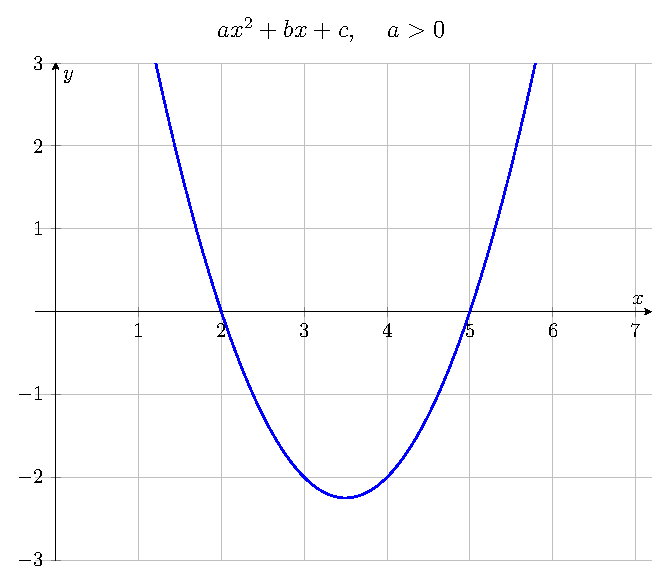
\includegraphics[height=12cm,page=1]{quadratic-parabola}
\end{figure}
The opposite is true: if $a<0$, the parabola has an inverted $U$-shape and a maximum in the positive range. Thus, the vertex is a minimum for $a>0$ and a maximum for $a<0$ (for $a=0$, the equation is linear and does not have a turning point). 

What if $\Delta<0$? In this case, there exist two complex roots. The formula above becomes:
\begin{align*}
r_1 = \frac{-b+i\sqrt{-\Delta}}{2a}
  \qquad
r_2 = \frac{-b-i\sqrt{-\Delta}}{2a} 
  \qquad\text{where}\quad i^2 = -1
\end{align*}
It is still true that
\begin{align*}
r_1 + r_2 
  & = \frac{-b}{a} \\
r_1 \times r_2 
  & = \frac{c}{a}
\end{align*}
Thus we can find the coordinates of the vertex without explicitly solving for the roots and without even knowing if the roots are real or complex, simply by carefully using the equation's coefficients:
\begin{align*}
x_{\text{vertex}} & = \frac{-b}{2a} \\
y_{\text{vertex}} & = c - \frac{b^2}{4a}
\end{align*}

An interesting special case is when $b^2=4ac$. This implies $\Delta=0$ and the equation admits a ``double'' root 
\begin{align*}
\Delta = 0 \quad\Rightarrow\quad r_1 = r_2 = \frac{-b}{2a}
\end{align*}
